Before the system can run properly some masks needs to be defined. These are used to:

\begin{itemize}
\item Define doors
\item Define non-interesting areas
\item Define entering checkpoints
\end{itemize}

These are adjusted in the Configure Window found under the System tab in the menu bar.

\subsubsection{Checkpoint circles}
The first thing to do is to insert three circles that are used as checkpoints when the system is counting people. All three circles needs to be passed before the system accepts it as and enter or exit. To draw a circle, check the circle check box. Place the cursor where want the center of your circle to be. Now press the mouse and move the cursor to adjust the radius. Three circles are automatically drawn and they should cover the door as shown in figure \ref{fig:circlePlacement} below.

\begin{figure}[H]
	\centering
	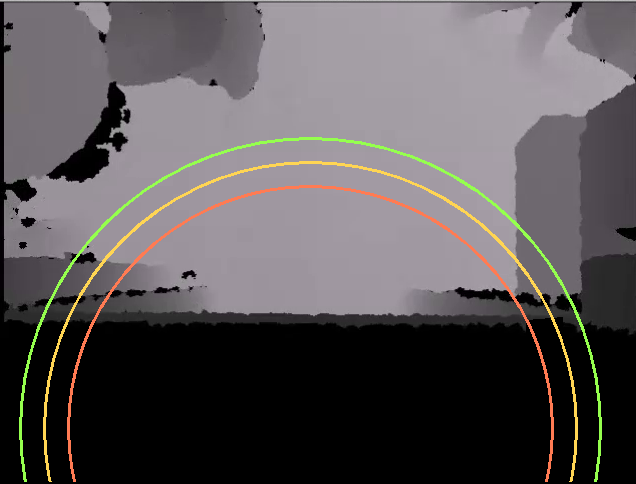
\includegraphics[width=\linewidth]{images/Manual2.png}
	\caption[Circle placment]{\textit{A preferred placement of the checkpoint circles. }}
	\label{fig:circlePlacement}  %Skapar referens till figuren
\end{figure}

\newpage
\subsubsection{Door mask}
The door mask should cover the entire door with some surrounding in front of the door. It is better to make this area too big rather than too small since people entering the room need to appear inside of this mask in order to be counted. A good example is shown in figure \ref{fig:doorMask} below. 

To add a door mask press \textit{New Polygon}. Now draw the mask by clicking in the image which adds control points to the mask, forming a polygon. To undo press Ctrl + Z. When the mask is done press \textit{Add as door}.

\begin{figure}[H]
	\centering
	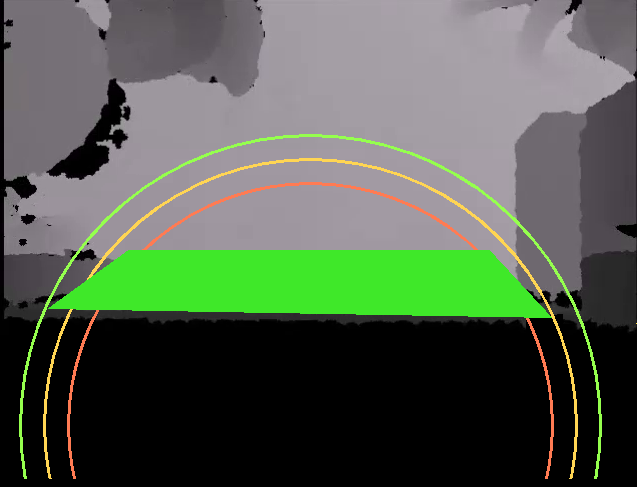
\includegraphics[width=\linewidth]{images/Manual3.png}
	\caption[Exclusion mask]{\textit{The preferred placement of the door mask is showed in green.}}
	\label{fig:doorMask}  %Skapar referens till figuren
\end{figure}

\newpage
\subsubsection{Exclusion mask}
Exclusion masks should cover areas that should be completely ignored by system e.g. where people can not walk or appear. This can be areas like tables or areas above the door (walls in this case). This is illustrated in figure \ref{fig:exMask} below. Note that for long usage of the system, movable furniture should not be excluded.

To add an exclusion mask press \textit{New Polygon}. Now draw the mask by clicking in the image which adds control points to the mask, forming a polygon. To undo press Ctrl + Z. When the mask is done press \textit{Add as exclusion}.

\begin{figure}[H]
	\centering
	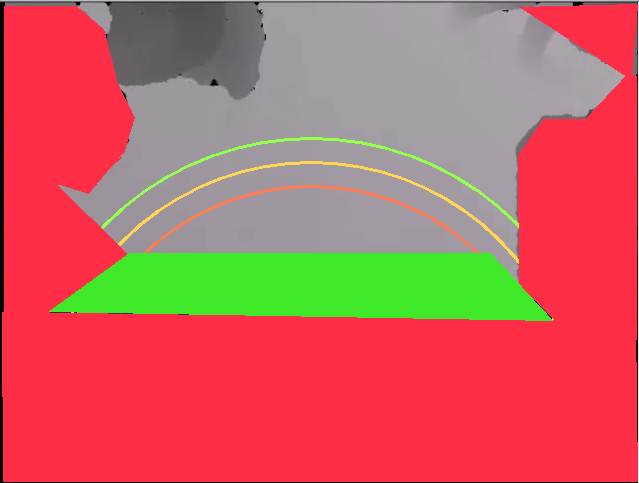
\includegraphics[width=\linewidth]{images/Manual1.png}
	\caption[Exclusion mask]{\textit{Exclusion mask is marked as red. It covers areas where people can not walk or appear.}}
	\label{fig:exMask}  %Skapar referens till figuren
\end{figure}

\newpage
\subsection{Configuration file}
The config file used by the algorithm pipeline is called \textit{mainConf.yml}. In it any configurable variable in any algorithm currently selected to be in the pipeline can be specified. The pipeline itself can also be specified, allowing fo rapid swapping of algorithms. The most useful variables in the current pipeline are shown in table \ref{table:commonVariables}.\\

\begin{table}[hbt]
	\begin{tabular}{ | l | l | p{7.5cm} | }
	    \hline
	    \textbf{Variable} & \textbf{Algorithm/Program-part} & \textbf{Description} \\ \hline
	    runFromFile & Network & If set to 1, the video sources are files found in the paths \textit{videoFilePaths}.  \\ \hline
	    videoFilePaths & Network & The paths to the video files used if running from file.  \\ \hline
	    useKinect & Network & If set to 1, the video sources are from Microsoft Kinect cameras. \\ \hline
	    TrackingMaximumDistance & Tracking & The maximum distance an object can be considered to have moved since last frame. \\ \hline
	    TrackingMinimzumLifeSpan & Tracking & The minimal time (in \# frames) a potential object must have existed (and been tracked) before it is considered a real object. \\ \hline
	    TrackingMaximumTimeLost & Tracking & The maximum time (in \# frames) an object is allowed to be lost before it is forgotten. \\ \hline
	    lowestDistanceOverFloor & Kinect Segmentation & The limit (height units) of how short a person can be. Set this variable using the GUI calibration utility described previously. \\ \hline
	    webServerUrl & Network & The address to the web service to which results are reported. \\ \hline
	    
	    lowOccupancyThreshold & Queue Severity Estimation & If there are more people than this and less than highOccupancyThreshold, queue severity will be set to 1 (medium). Setting these value is optional but recommended for rooms where an overwhelming proportion of the occupants will be in a queue (e.g. rooms without places for sitting). If no values are set the severity is solely determined by visible queues. \\ \hline
	    
	    highOccupancyThreshold & Queue Severity Estimation & If there are more people than this, queue severity is 2 (high). This value must be higher than lowOccupancyThreshold if set. \\ \hline
	    
	\end{tabular}
	\label{table:commonVariables}
	\caption{The most useful and common variables in the current pipeline.}
\end{table}

\newpage
Currently the pipeline consists of two major algorithms: \textit{ImageProcessor} and \textit{Analytics}. These in turn have several sub-algorithms that are executed in the order specified in the config file. The current pipeline is structured in the following way: \\
\hspace*{0.5cm}\textit{ImageProcessor:\\
\hspace*{1cm}- KinectSegmentation\\
\hspace*{1cm}- TrackingBruteForce}\\
\hspace*{0.5cm}\textit{Analytics:\\
\hspace*{1cm}- EntryExitCounter\\
\hspace*{1cm}- FlowEstimator\\
\hspace*{1cm}- QueDetector\\
\hspace*{1cm}- QueSeverityEstimator}\\\\
Any algorithm registed in the system can be used as a subalgorithm for any other algorithm, writing in the config file in the same way as with \textit{KinectSegmentation} being a sub algorithm to \textit{ImageProcessor}. To get an empty algorithm placeholder any none-registerd algorithm name (or variable name) may be used, such as:\\
\hspace*{0.5cm}\textit{UnregisterdName:\\
\hspace*{1cm}- KinectSegmentation\\
\hspace*{1cm}- ...}\\
It can now be used as a sub-algorithm to another algorithm (or placeholder algorithm):\\
\hspace*{0.5cm}\textit{ImageProcessors:\\
\hspace*{1cm}- UnregisterdName\\
\hspace*{1cm}- ...}\\
A placeholder algorithm works by just passing through initialization and processing calls to its sub-algorithms.\\\\
\textbf{Warning: If you do not know what your are doing, do not modify the algorithm pipeline. Some algorithms have requirements which must be provided by earlier algorithms, the system will not run if these are not met. See the code documentation for further details on requirements and effetcs of different algorithms.}

